\documentclass{artikel1}

\title{Žraloky: Majstri oceánov}
\author{Denisa Rudincová}

\usepackage[english, slovak]{babel}
\usepackage[resetfonts]{cmap}
\usepackage{lmodern}
\usepackage[utf8]{inputenc}
\usepackage[T1]{fontenc}
\usepackage{graphicx}
\usepackage{pdfpages}
\usepackage[xindy]{imakeidx}  % potrebné pridať [noautomatic], pretože inak na tom pracujem v overleafe
\usepackage{microtype}


\usepackage{hyperref}
\usepackage[backend=biber,
            style=alphabetic,
            maxnames=5,
            alldates=iso,
            seconds=true]{biblatex}

\addbibresource{databaza_literatury.bib}
\makeindex[options=-L slovak-large -C utf8]

\begin{document}

% životopis
\includepdf[linktodoc=true,pages=-]{zivotopis.pdf}

% povídačky o žralokoch
\maketitle
\tableofcontents

\section{Úvod}
Žraloky\index{žraloky@žralok} patria medzi najfascinujúcejšie tvory oceánov a~predstavujú záhadné a~neustále skúmané bytosti v~rámci morského ekosystému\index{ekosystém}. Ich jedinečné fyziologické a~behaviorálne vlastnosti si zaslúžia pozornosť vedeckej komunity a~verejnosti zároveň. Sú jedny z~najstarších a~najvývojovejších druhov rýb, ktoré obývajú svetové oceány viac než 400 miliónov rokov.

\section{Biológia žralokov}

\subsection{Štruktúra tela a~fyziológia\index{fyziológia}}
Žraloky majú charakteristickú stavbu tela, ktorá zahŕňa skelet\index{skelet} tvorený chrupavkou namiesto kostí. Táto anatómia im umožňuje byť obratnými a~rýchlymi lovcami, čo je nevyhnutné pre ich prežitie v~náročných oceánskych prostrediach. Srdce\index{srdce} žralokov je obzvlášť efektívne, čo podporuje ich vytrvalosť a~schopnosť podniknúť rozsiahle migračné trasy.

\begin{figure}
  \begin{center}
  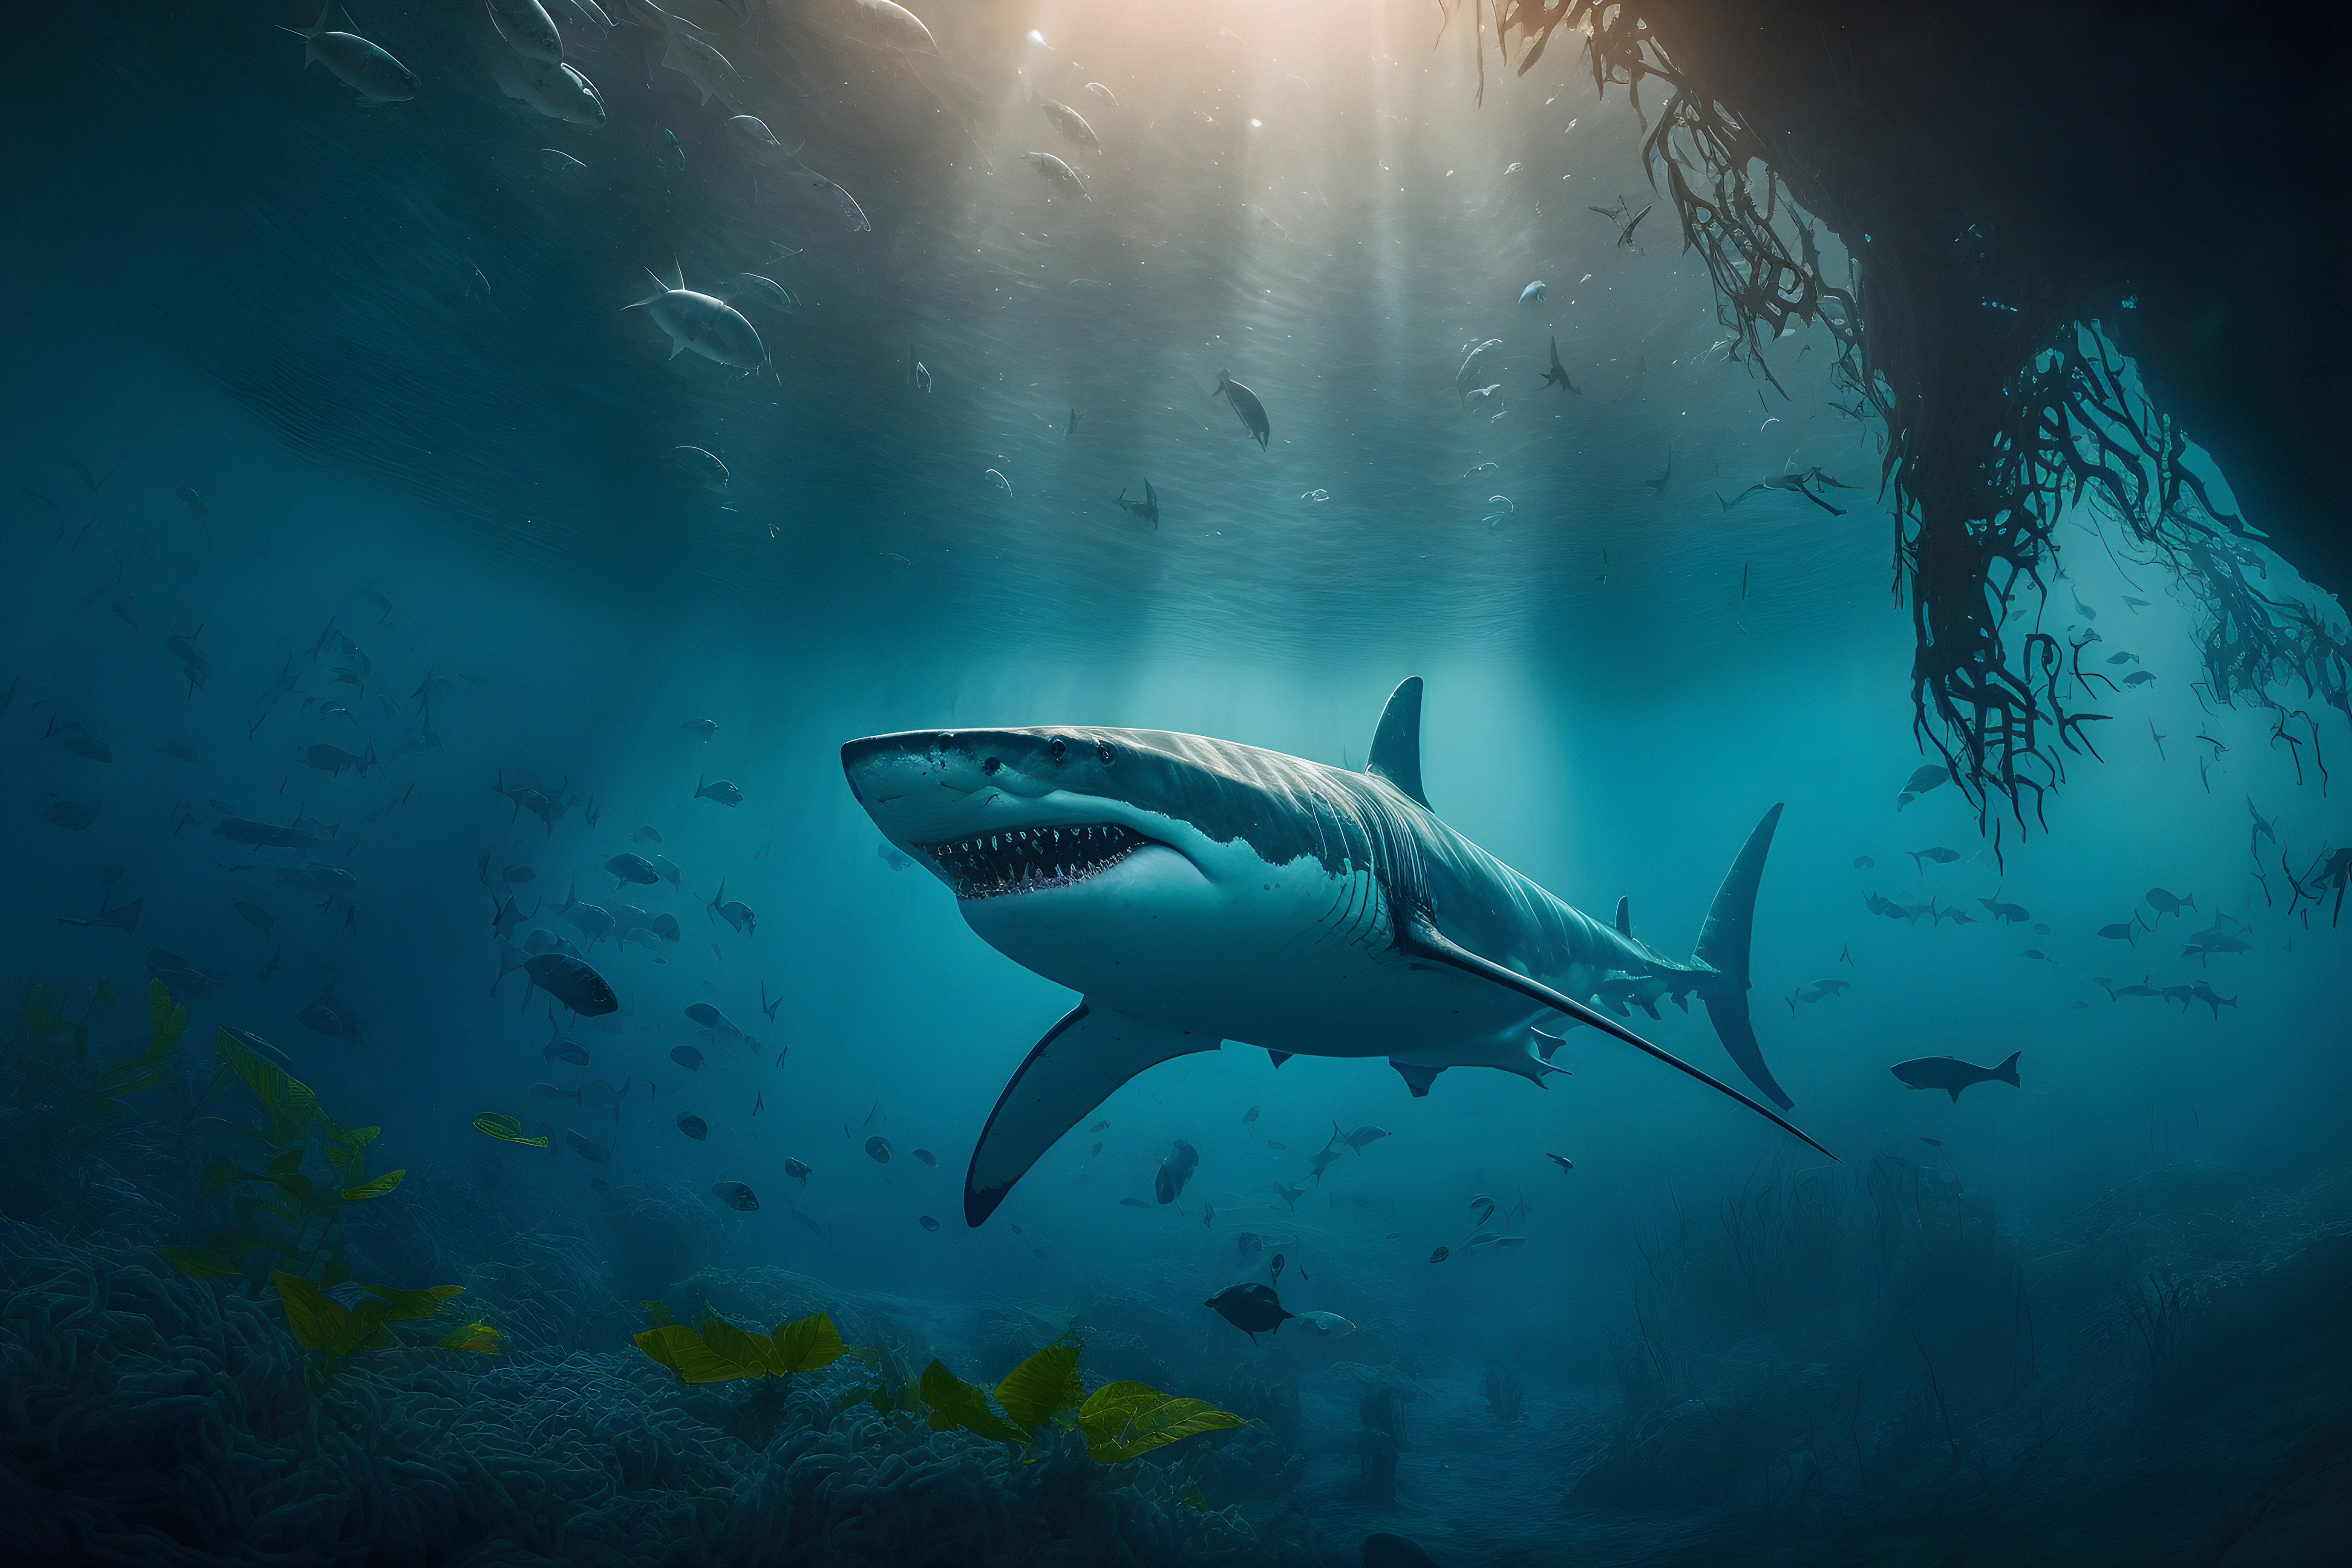
\includegraphics[width=1\textwidth]{shark4.jpg}
  \caption{Žralok modrý (Carcharodon carcharias)}
  \label{shark4}
  \end{center}
\end{figure}

\subsection{Zmysly}
Žraloky majú vynikajúce zmysly, ktoré im umožňujú efektívne loviť potravu a~navigovať v~oceáne\index{oceáne@oceán}. Ich čuch\index{čuch} je mimoriadne citlivý, pričom niektoré druhy dokážu detekovať krv vo vode na veľké vzdialenosti. Elektrorecepčný systém\index{elektrorecepčný systém} žralokov im umožňuje zachytávať slabé elektrické polia, čo je užitočné pri hľadaní koristi v~oceáne. \cite{senses}

\subsection{Reprodukcia a~rast}
Žraloky majú rôzne stratégie reprodukcie\index{reprodukcia}. Niektoré druhy sú vajcoživorodé\index{vajcoživorodosť}, čo znamená, že sa vajíčka vyvíjajú vo vnútri matky a~liahnu sa hneď pre pôrodom, alebo po ňom. U~iných druhov samice kladú vajíčka, ktoré sa potom vyvíjajú mimo maternice.

Rast žralokov je často pomalý a~mnohé druhy dosahujú pohlavnú zrelosť až po niekoľkých rokoch. Táto pomalá reprodukcia znamená, že populácie žralokov sú náchylné na nadmerný rybolov a~môžu mať obmedzenú schopnosť zotaviť sa z~úbytkov.

\section{Ekologická úloha žralokov}
Žraloky sú kľúčovými predátormi v~morských ekosystémoch, čím regulujú populácie rýb a~udržiavajú ekologickú rovnováhu. Výskum ukázal, že pokles populácií žralokov môže viesť k~nerovnováhe v~oceánskych komunitách a~nekontrolovateľnému rozmnožovaniu niektorých druhov rýb.

Podľa profesora Johna Smitha, odborníka na morskú ekológiu, je ochrana žralokov nevyhnutná pre udržanie zdravia morských ekosystémov. Ich úloha v~regulácii populácií morských organizmov je nepochybná. \cite{decline}

\section{Aktuálne hrozby a~ochrana}
Žiaľ, žraloky čelia vážnym hrozbám zľudovaním ich životného prostredia, nadmerným rybolovom a~lovenímp pomocou plávajúcich sietí. Organizácie zaoberajúce sa ochranou životného prostredia sa snažia zdôrazniť dôležitosť zachovania žralokov a~presadzovať legislatívu na ochranu týchto ohrozených druhov.

Ako uviedla Dr. Sarah Johnson, špecialistka na ochranu morského prostredia, je kľúčové vytvoriť medzinárodné dohody na reguláciu rybolovu a~presadiť prísne opatrenia na ochranu žralokov a~ich životných prostredí. \cite{conservation}

\begin{figure}
  \begin{center}
  \includegraphics[width=1\textwidth]{shark3.eps}
  \caption{Vektorový žralok}
  \label{shark3}
  \end{center}
\end{figure}

\section{Záver}
Žraloky predstavujú fascinujúce bytosti, ktoré majú kľúčový význam pre ekologickú rovnováhu oceánov. Ich ochrana a~zachovanie sú nevyhnutné pre udržanie biodiverzity\index{biodiverzita} a~zachovanie morských ekosystémov. Vedci a~ochranári spolupracujú s~cieľom presadiť opatrenia, ktoré zabezpečia budúcnosť týchto majstrov oceánov.

\printbibliography[heading=bibintoc]

\printindex
\begin{figure}
  \begin{center}
  \includegraphics[width=0.7\textwidth]{shark2.eps}
  \caption{Ďalší vektorový žralok}
  \label{shark2}
  \end{center}
\end{figure}

\end{document}
